\documentclass[12pt]{article}
%\usepackage[utf8]{inputenc}
%\documentclass[UTF8]{ctexart}
%\usepackage[UTF8, heading = false, scheme = plain]{ctex}
\usepackage{geometry}
%geometry{a4paper,scale=0.9}
\geometry{a4paper,left=1cm,right=1cm,top=1cm,bottom=2cm}
\usepackage{amsfonts}
\usepackage{color}
\usepackage{url}
%\usepackage{biblatex}
\usepackage{amsmath}
\usepackage{amssymb}
\usepackage{latexsym}
\usepackage{cite}
%\addbibresource{ref.bib}
%\bibliography{ref.bib}
\usepackage{caption}
\usepackage{graphicx, subfig}
\usepackage{float}
%\usepackage[fontset=ubuntu]{ctex}
%\usepackage{fontspec}
\usepackage{xeCJK}
%\usepackage[colorlinks,
%anchorcolor=black,
%citecolor=black]{hyperref}
%\setmainfont{SimSun}
\usepackage[section]{placeins}
\usepackage{enumitem}
\usepackage{framed}
\usepackage[framemethod=TikZ]{mdframed}
\usepackage{indentfirst}
\usepackage{setspace}%使用间距宏包
\linespread{1.5}
%\title{预备知识}
%\author{leolinuxer }
%\date{June 2020}

\title{蒙特卡洛树搜索(MCTS)\cite{Fundation_Of_MCTS_In_28_Days}\cite{MCTS_Introduction_Briefly}}
%\author{leolinuxer }
%\date{June 2020}

\begin{document}
\maketitle

\section{极小极大(Minimax)搜索}
先看传统的博弈游戏树搜索,著名的\textbf{极小极大(Minimax)搜索},学过算法的朋友会清楚。看下图,假设现在轮到黑棋,黑棋有b1和b2两手可选,白棋对于b1有w1/w2两手可选,白棋对于b2有w3/w4/w5三手可选:
\begin{figure}[H]
    \centering
    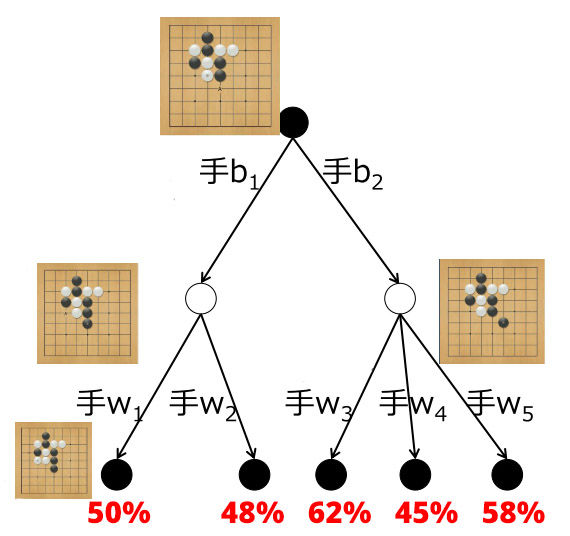
\includegraphics[width=.5\textwidth]{fig/MCTS-Minimax-Search-Example.jpg}
\end{figure}

然后假设走完w1/w2/w3/w4/w5后,经过局面评估,黑棋的未来胜率分别是 50\%/48\%/62\%/45\%/58\%(等一下,这些胜率是怎么评估出来的?我们后文会说这个问题)。

请问,黑棋此时最佳的着法是b1还是b2?如果是用\textbf{蒙特卡洛方法,趋近的会是其下所有胜率的平均值}。例如经过蒙特卡洛模拟,会发现b1后续的胜率是49\% = (50+48)/2,而b2后续的胜率是55\% = (62+45+58)/3。

于是蒙特卡洛方法说应该走b2,因为55\%比49\%的胜率高。但这是错误的。因为如果白棋够聪明,会在黑棋走b1的时候回应以w2(尽量降低黑棋的胜率),在黑棋走b2的时候回应以w4(尽量降低黑棋的胜率)。

所以走b1后黑棋的真实胜率是48\%,走b2后黑棋的真实胜率是45\%。黑棋的正解是b1。这就是 Minimax 搜索的核心思想:\textbf{在搜索树中,每次轮到黑棋走时,走对黑棋最有利的;轮到白棋走时,走对黑棋最不利的。}由于围棋是零和游戏,这就可以达到最优解。这是一个由底往上的过程:先把搜索树画到我们可以承受的深度,然后逐层往上取最大值或最小值回溯,就可以看到双方的正解(如果胜率评估是准确的)。而实际编程的时候,是往下不断生长节点,然后动态更新每个父节点的胜率值。

下图是一个更多层的例子:
\begin{figure}[H]
    \centering
    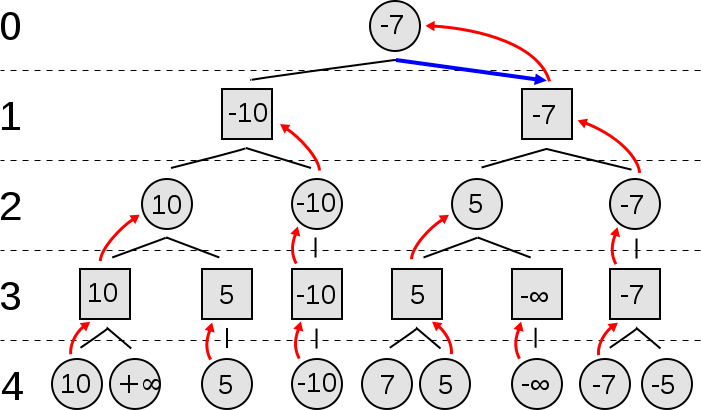
\includegraphics[width=.5\textwidth]{fig/MCTS-Minimax-Search-Multiple-Layers.png}
\end{figure}

值得注意的是,在实际对局中,胜率评估会有不准确的地方,这就会导致“地平线效应”,即由于电脑思考的深度不够,且胜率评估不够准确,因此没有看见正解。

\section{蒙特卡洛方法}
首先注意,\textbf{蒙特卡洛方法和蒙特卡洛树搜索不是同一种算法}。

\textbf{蒙特卡洛法方法是评判棋盘局面的一种方法}。因为围棋很难写出好的估值函数,于是上世纪有人提出了一种神奇的方法:双方在某个局面下「随机」走子,注意是「随机」走,走到终局或者残局为止,随机很多次(比如一万盘),计算胜率,胜率越高的局面就越好,不用写极其复杂的估值函数,然后就套用博弈树的最大最小算法即可。

但其实这是个伪算法,就举个极端的例子,比如说我下某步棋之后,对方有 100 种应对—— 99 种会导致劣势,但是有 1 种必胜下法,我就绝对不能下这步棋。但是「蒙特卡洛树搜索」是个真算法,并且它其实在 alphago 之前早就有了,而且能胜业余的段级选手,在当时是很大的突破。

\section{蒙特卡洛树搜索}
蒙特卡洛树搜索(简称 MCTS)是 Rémi Coulom 在 2006 年在它的围棋人机对战引擎 「Crazy Stone」中首次发明并使用的的 ,并且取得了很好的效果。

\subsection{蒙特卡洛树搜索和蒙特卡洛方法的区别}
\begin{enumerate}
\setlength{\itemsep}{0pt}
\setlength{\parsep}{0pt}
\setlength{\parskip}{0pt}
    \item 如果用蒙特卡洛方法做上一百万次模拟,b1和b2的胜率仍然会固定在49\%和55\%,不会进步,永远错误。所以它的结果存在偏差(Bias),当然,也有方差(Variance)。
    \item 而蒙特卡洛树搜索在一段时间模拟后,b1和b2的胜率就会向48\%和45\%收敛,从而给出正确的答案。所以它的结果不存在偏差(Bias),只存在方差(Variance)。但是,对于复杂的局面,它仍然有可能长期陷入陷阱,直到很久之后才开始收敛到正确答案。
\end{enumerate}

如果想把 Minimax 搜索运用到围棋上,立刻会遇到两个大问题:
\begin{enumerate}
\setlength{\itemsep}{0pt}
\setlength{\parsep}{0pt}
\setlength{\parskip}{0pt}
    \item \textbf{搜索树太广}。棋盘太大了,每一方在每一步都有很多着法可选。
    \item \textbf{很难评估胜率}。除非把搜索树走到终局,这意味着要走够三百多步(因为对于电脑来说,甚至很难判断何时才是双方都同意的终局,所以只能傻傻地填子,一直到双方都真的没地方可以走为止)。简单地说,搜索树也需要特别深。
\end{enumerate}

\subsection{蒙特卡洛树搜索详解}
蒙特卡洛树搜索的意义在于部分解决了上述两个问题:
\begin{enumerate}
\setlength{\itemsep}{0pt}
\setlength{\parsep}{0pt}
\setlength{\parskip}{0pt}
    \item \textbf{它可以给出一个局面评估,虽然不准,但比没有强}。这就部分解决了第二个问题。
    \item \textbf{根据它的设计,搜索树会较好地自动集中到“更值得搜索的变化”}(注意,也不一定准)。如果发现一个不错的着法,蒙特卡洛树搜索会较快地把它看到很深,可以说它结合了广度优先搜索和深度优先搜索,类似于启发式搜索。这就部分解决了第一个问题。
\end{enumerate}

最后,随着搜索树的自动生长,蒙特卡洛树搜索可以保证在足够长的时间后收敛到完美解(但可能需要极长的时间)。下面看具体过程(重复千千万万次):
\begin{figure}[H]
    \centering
    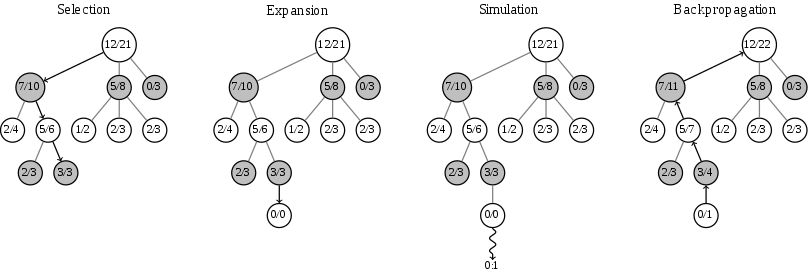
\includegraphics[width=1\textwidth]{fig/MonteCarlo-Tree-Search-4-Steps.png}
\end{figure}

上图中每个节点代表一个局面。而 A/B 代表这个节点被访问 B 次,黑棋胜利了 A 次。例如一开始的根节点是 12/21,代表总共模拟了 21 次,黑棋胜利了 12 次。

从图中可以看出,蒙特卡洛树搜索分位四步:
\begin{enumerate}
\setlength{\itemsep}{0pt}
\setlength{\parsep}{0pt}
\setlength{\parskip}{0pt}
    \item \textbf{选择(Selection)}。  我们将节点分成三类:(1)未访问:还没有评估过当前局面;(2)未完全展开:被评估过至少一次,但是子节点(下一步的局面)没有被全部访问过,可以进一步扩展;(3)完全展开:子节点被全部访问过。从根节点往下走,每次都选一个“最值得看的子节点”(具体规则稍后说),直到来到一个“存在未扩展的子节点”的节点,如图中的 3/3 节点。什么叫做“存在未扩展的子节点”,其实就是指这个局面存在未走过的后续着法。
    \item \textbf{扩展(Expansion)}。我们给这个节点加上一个 0/0 子节点,对应之前所说的“未扩展的子节点”,就是还没有试过的一个着法。
    \item \textbf{模拟(Simluation)}。从上面这个没有试过的着法开始,用快速走子策略(Rollout policy)走到底,得到一个胜负结果。按照普遍的观点,快速走子策略适合选择一个棋力很弱但走子很快的策略。因为如果这个策略走得慢(比如用 AlphaGo 的策略网络走棋),虽然棋力会更强,结果会更准确,但由于耗时多了,在单位时间内的模拟次数就少了,所以不一定会棋力更强,有可能会更弱。这也是为什么我们一般只模拟一次,因为如果模拟多次,虽然更准确,但更慢。
    \item \textbf{回溯(Backpropagation)}。把模拟的结果加到它的所有父节点上。例如第三步模拟的结果是 0/1(代表黑棋失败),那么就把这个节点的所有父节点加上 0/1。
\end{enumerate}

\subsection{选择节点的方法}
怎么选择节点?和从前一样:\textbf{如果轮到黑棋走,就选对于黑棋有利的;如果轮到白棋走,就选对于黑棋最不利的。但不能太贪心,不能每次都只选择“最有利的/最不利的”,因为这会意味着搜索树的广度不够,容易忽略实际更好的选择。}这是因为如果一开始在某个节点进行模拟的时候,尽管这个节点不怎么好,但是一开始随机走子的时候赢了一盘,就会一直走这个节点了。

因此人们造了一个函数
$$
\mathbb{UCT}(v_i, v)  = \frac{Q(v_i)}{N(v_i)} + C \cdot \sqrt{\frac{\log(N(v))}{N(v_i)}}
$$

其中,$Q(v)$ 是该节点赢的次数,$N(v)$ 是该节点模拟的次数,$C$ 是一个常数。或者说是这样的:
$$
score = x_{child} + C \cdot \sqrt{\frac{\log(N_{parent})}{N_{child}}}
$$

其中 $x$ 是节点的当前胜率估计(注意,如前所述,要考虑当前是黑棋走还是白棋走!),$N$ 是节点的访问次数。$C$ 是一个常数。$C$ 越大就越偏向于广度搜索,$C$ 越小就越偏向于深度搜索。

我们看例子说明这是什么意思,就看之前的图吧。假设根节点是轮到黑棋走。那么我们首先需要在 7/10、5/8、0/3 之间选择:
\begin{enumerate}
\setlength{\itemsep}{0pt}
\setlength{\parsep}{0pt}
\setlength{\parskip}{0pt}
    \item 其中 7/10 对应的分数为:$7/10 + C\cdot\sqrt{\frac{\log{21}}{10}} \approx 0.7 + 0.55C$
    \item 其中 5/8 对应的分数为:$5/8 + C\cdot\sqrt{\frac{\log{21}}{8}} \approx 0.625 + 0.52C$
    \item 其中 0/3 对应的分数为:$0/3 + C\cdot\sqrt{\frac{\log{21}}{3}} \approx 0 + 1.00C$ 
\end{enumerate}
可以注意到,$C$越大,就会越照顾访问次数相对较少的子节点。如果 $C$ 比较小,我们将会选择 7/10,接着就要在 2/4 和 5/6 间选择。注意,由于现在是白棋走,需要把胜率估计倒过来:
\begin{enumerate}
\setlength{\itemsep}{0pt}
\setlength{\parsep}{0pt}
\setlength{\parskip}{0pt}
    \item 其中 2/4 对应的分数为:$(1-2/4) + C\cdot\sqrt{\frac{\log{10}}{4}} \approx 0.5+0.76C$
    \item 其中 5/6 对应的分数为:$(1-5/6) + C\cdot\sqrt{\frac{\log{10}}{6}} \approx 0.17+0.62C$
\end{enumerate}

那么我们下一步肯定应该选 2/4。

最后,AlphaGo 的策略网络,可以用于改进上述的分数公式,让我们更准确地选择需扩展的节点。而 AlphaGo 的价值网络,可以与快速走子策略的模拟结果相结合,得到更准确的局面评估结果。注意,如果想写出高效的程序,这里还有很多细节,因为策略网络和价值网络的运行毕竟需要时间,我们不希望等到网络给出结果再进行下一步,在等的时候可以先做其它事情,例如 AlphaGo 还有一个所谓 Tree policy,是在策略网络给出结果之前先用着。


\subsection{选择终止的方法(得到最佳走法)}
一般来说\textbf{最佳走法就是具有最高访问次数的节点},这点可能稍微有点反直觉。这样评估的原因是因为蒙特卡洛树搜索算法的核心就是,越优秀的节点,越有可能走,反过来就是,走得越多的节点,越优秀。也就是说,\textbf{最终应该选择访问量最大的节点,而不是胜率最高的节点}。

\subsection{AlphaGo 对 MCTS 的改进}
deepmind 将 MCTS 和近年来取得突破性进展的神经网络结合起来,主要是针对上面两个步骤作了改进:
\begin{enumerate}
\setlength{\itemsep}{0pt}
\setlength{\parsep}{0pt}
\setlength{\parskip}{0pt}
    \item \textbf{模拟}:首先上面四步里,最玄学、感觉最不靠谱的一步是「模拟」,用随机快速走子的方法走完一盘棋,然后记录胜盘和下了多少盘,这一步虽然是蒙特卡洛树搜索的核心,但是并不那么准确。在 Alphago Lee 中,叶子节点的估值是两个部分的加权和:(1)一种带有手工特征的浅层 softmax 神经网络:采用自定义快速走棋策略的标准走棋评估;(2)估值网络:基于 13 层卷积神经网络的位置评估,训练自 Alpha Go 自我对弈的三千万个不同位置(没有任何两个点来自同一场游戏);而 alphago zero 迈出了更远的一步,他们根本就不进行模拟,而是用一个 19 层 CNN 残差神经网络直接评估当前节点。(神经网络可以输出位置评估,得出每个位置的概率向量)。也就是说,\textbf{利用神经网络,无需模拟,直接能算出每个位置的概率},可以说是直接消除了玄学问题。
    \item \textbf{选择}:既然已经不是真的通过「模拟」的出赢的次数和已经评估的次数,那么我们之前通过 UCT 值的大小来向下搜索、选择一个未访问的叶子节点的方法也需要作出相应修改。函数变为:
$$
\mathbb{UCT}(v_i, v) = \frac{Q(v_i)}{N(v_i)} + C\cdot P(v, v_i)\sqrt{\frac{N(v)}{1+N(v_i)}}
$$
其中 $UCT(v_i, v)$ 表示从状态(节点) $v_i$ 转移到 $v$ 的价值评估,$P(v_i, v)$表示从状态 $v_i$ 转移到 $v$ 的概率,或者用一个术语叫做「移动的先验概率」,这个概率是用策略网络训练出来的,基于人类游戏数据集的受监督学习。而在 Alphago Zero 中只有一个网络,它既是估值网络也是策略网络。它完全通过从随机初始状态开始进行自我对弈训练。并行训练多个网络,在每个检查点,基于当前最优的神经网络,评选出最优的网络用来生成训练数据。
\end{enumerate}

\section{扩展阅读}
推荐蒙特卡罗树搜索的论文 A Survey of Monte Carlo Tree Search Methods


%\printbibliography
\bibliography{../ref}
\bibliographystyle{IEEEtran}
\end{document}